% !TeX program = pdflatex
% =============================================================
% Public Economics -- Lecture 4
% Taxation
% Based on: Gruber, J. "Public Finance and Public Policy", Ch. 18
%           (18.1, 18.3, 18.4, 18.5)
%           Leenders, W. "Microeconomics of Public Policy, Part IV:
%           Taxation" (Sciences Po, MPA 2023-2024)
% Austrian institutional and empirical context added for WU Vienna.
% =============================================================
\documentclass[11pt,aspectratio=169]{beamer}

\usetheme{metropolis}
\usepackage[utf8]{inputenc}
\usepackage[T1]{fontenc}
\usepackage{lmodern}
\usepackage{booktabs}
\usepackage{array}
\usepackage{textcomp}
\usepackage{siunitx}
\usepackage{tikz}
\usepackage{pgfplots}
\pgfplotsset{compat=1.18}
\usepackage{pgf-pie}
\usetikzlibrary{positioning,arrows.meta,calc}

% ----------------------------------------------------------------
% Colors: WU Vienna blue as primary accent
% ----------------------------------------------------------------
\definecolor{wublue}{HTML}{003D7C}
\definecolor{wulight}{HTML}{4F8FC4}
\definecolor{wugray}{HTML}{5C6670}
\definecolor{wured}{HTML}{B0202E}
\definecolor{wugreen}{HTML}{4C8C6B}
\definecolor{wuyellow}{HTML}{D9A441}
\setbeamercolor{palette primary}{bg=wublue,fg=white}
\setbeamercolor{frametitle}{bg=wublue,fg=white}
\setbeamercolor{progress bar}{fg=wublue,bg=wulight!30}
\setbeamercolor{alerted text}{fg=wured}

\setbeamertemplate{frame footer}{Taxation}
\setbeamertemplate{footline}[frame number]

\title{Public Economics}
\subtitle{Lecture 4 \(\cdot\) Taxation}
\author{Shushanik Margaryan}
\institute{WU Vienna University of Economics and Business}
\date{Winter Term}

% Source note command for footnote-style citations on data slides
\newcommand{\srcnote}[1]{{\footnotesize\color{wugray}Source: #1}}

\begin{document}

% =============================================================
\begin{frame}
  \titlepage
\end{frame}

\begin{frame}{Today's Questions}
  \begin{itemize}
    \item What are the different types of taxes governments levy, and how does the burden of a tax actually get shared between buyers and sellers?
    \item What does it mean for a tax system to be ``fair,'' and how do we measure that?
 
  \end{itemize}
  \vspace{1em}
  \begin{block}{Based on}
    Gruber, J. \emph{Public Finance and Public Policy}, Ch.\ 18  
  \end{block}
\end{frame}

% =============================================================
\begin{frame}{Outline}
  \tableofcontents
\end{frame}

% =============================================================
\section{4.1 Types of Taxation}

\begin{frame}{Five Types of Taxes}
  \small
  \begin{itemize}
    \item \textbf{Payroll tax}: levied on earnings from work; finances social insurance (pensions, unemployment, health).
    \item \textbf{Individual income tax}: paid on income accrued during the year --- a broader base than payroll (interest, etc.) and often assessed per household, not per worker.
    \item \textbf{Corporate income tax}: levied on corporate earnings, to catch capital income that might otherwise escape individual-level taxation.
    \item \textbf{Wealth taxes}: levied on the \emph{value of assets} held (not income), e.g.\ property tax, estate/inheritance tax.
    \item \textbf{Consumption taxes}: levied on spending, e.g.\ VAT/sales tax; when applied to one specific good (fuel, tobacco, alcohol), called an \textbf{excise tax}.
  \end{itemize}
  \vspace{0.3em}
  \centering

\end{frame}

\begin{frame}{The Same Five Types, in Austria}
  \scriptsize
  \begin{center}
  \begin{tabular}{@{}p{2.6cm}p{9.3cm}@{}}
    \toprule
    \textbf{Type} & \textbf{Austrian tax(es)} \\
    \midrule
    Payroll & \emph{Sozialversicherungsbeiträge} --- pension, health, unemployment, accident insurance; split employer/employee \\[0.2em]
    Individual income & \emph{Einkommensteuer} (self-employment/business income); \emph{Lohnsteuer} (withholding on wage income) \\[0.2em]
    Corporate income & \emph{Körperschaftsteuer} (KSt) \\[0.2em]
    Wealth & \emph{Grundsteuer} (property) and \emph{Grunderwerbsteuer} (real-estate transfer) still exist; \emph{Vermögensteuer} and \emph{Erbschafts-/Schenkungssteuer} do \textbf{not} \\[0.2em]
    Consumption & \emph{Umsatzsteuer} (VAT); excise: \emph{Mineralölsteuer} (fuel), \emph{Tabaksteuer}, \emph{Alkohol-/Biersteuer}, \emph{NoVA} (vehicles), \emph{CO\textsubscript{2}-Bepreisung} (since 2022) \\
    \bottomrule
  \end{tabular}
  \end{center}
  \centering
   
\end{frame}

\begin{frame}{International Tax Revenues by Type}
\centering



		\textbf{OECD average}\\[0.2em]
			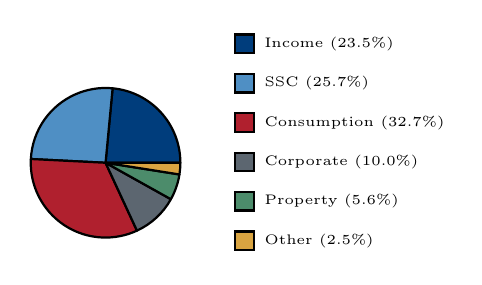
\begin{tikzpicture}
				\pie[
				radius=0.95, text=legend, hide number, font=\tiny,
				color={wublue,wulight,wured,wugray,wugreen,wuyellow}
				]{
					23.5/Income (23.5\%),
					25.7/SSC (25.7\%),
					32.7/Consumption (32.7\%),
					10.0/Corporate (10.0\%),
					5.6/Property (5.6\%),
					2.5/Other (2.5\%)
				}
			\end{tikzpicture}

\end{frame}

\begin{frame}{Taxation Around the World: Tax Revenue Composition}
  \begin{center}
    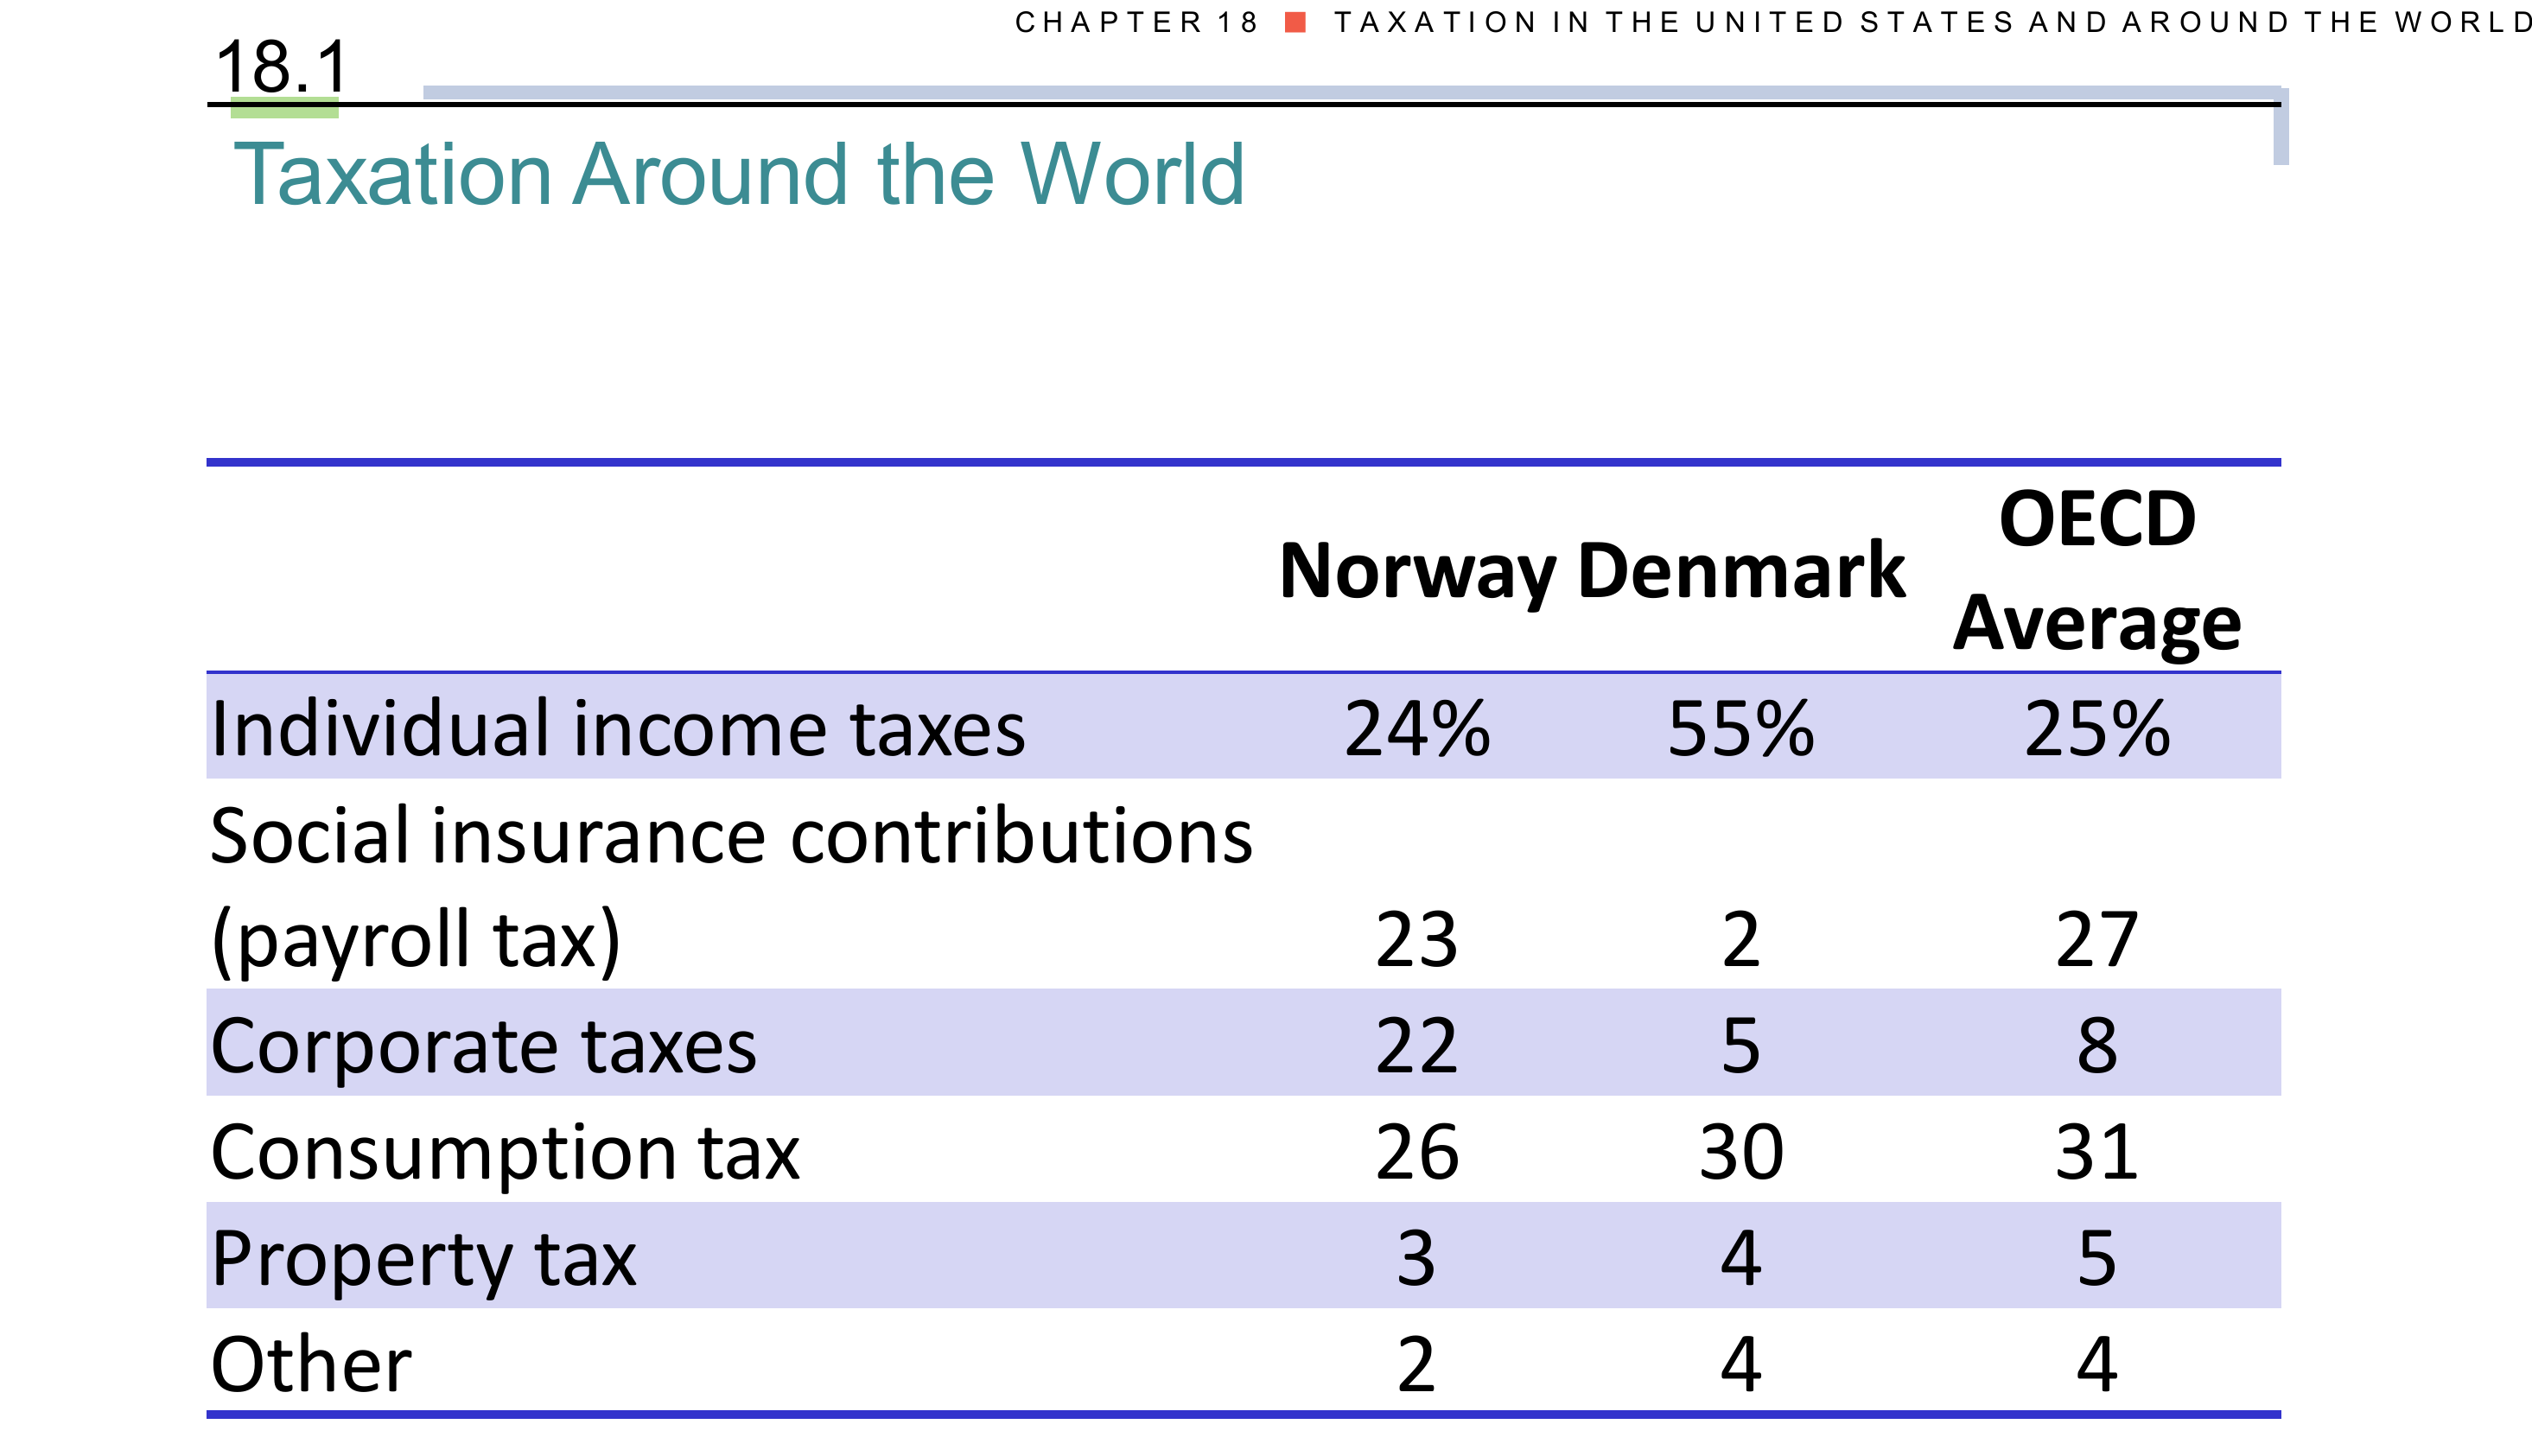
\includegraphics[height=4.55cm]{figures/taxation_around_world_norway_denmark_oecd.png}
  \end{center}
  \centering
  Two very different high-tax countries: Norway spreads revenue broadly across income, payroll, and corporate taxes; Denmark relies overwhelmingly on the individual income tax alone.\\
  \srcnote{Gruber, \emph{Public Finance and Public Policy}, \S18.1, ``Taxation Around the World.''}
\end{frame}

\begin{frame}{Where Does Austria Fit?}
  \begin{itemize}
    \item  Austria's tax mix leans heavily on \textbf{labor} 
    \item  Austria abolished its general \textbf{wealth tax} (\emph{Vermögensteuer}) in 1994, and its \textbf{inheritance/gift tax} lapsed in 2008 after the \emph{Verfassungsgerichtshof} ruled the property-valuation method unconstitutional and no replacement was passed. 
    \item Austria has had \emph{no} wealth or inheritance tax since.
  \end{itemize}
 
\end{frame}

% =============================================================
\section{4.2 Tax Incidence}

\begin{frame}{Tax Incidence: Who Really Pays?}
  \begin{block}{Tax incidence}
   Tax incidence measures who bears the legal or economic burden of a tax.
  \end{block}
  \vspace{0.3em}
  \begin{itemize}
    \item \textbf{Legal (statutory) incidence}: who is legally required to send the tax payment to the government.
    \item \textbf{Economic incidence}: who actually bears the burden, once prices adjust.
  \end{itemize}
 

\end{frame}

\begin{frame}{The Canonical Case: An Excise Tax}
  \begin{center}
  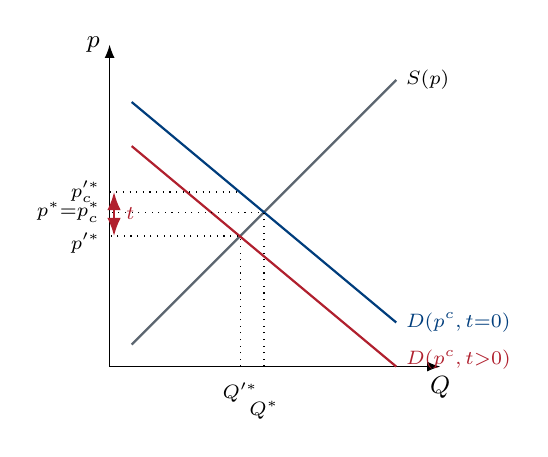
\begin{tikzpicture}[scale=0.56]
    \draw[-{Latex}] (0,0) -- (7.5,0) node[below, font=\small]{$Q$};
    \draw[-{Latex}] (0,0) -- (0,7.3) node[left, font=\small]{$p$};
    \draw[wugray, thick] (0.5,0.5) -- (6.5,6.5);
    \node[right, font=\scriptsize] at (6.5,6.5) {$S(p)$};
    \draw[wublue, thick] (0.5,6) -- (6.5,1);
    \node[right, font=\scriptsize, wublue] at (6.5,1) {$D(p^c,t{=}0)$};
    \draw[wured, thick] (0.5,5) -- (6.5,0);
    \node[right, font=\scriptsize, wured] at (6.5,0.15) {$D(p^c,t{>}0)$};
    \draw[dotted] (3.5,0) -- (3.5,3.5) -- (0,3.5);
    \draw[dotted] (2.96,0) -- (2.96,2.96) -- (0,2.96);
    \draw[dotted] (0,3.96) -- (2.96,3.96);
    \draw[wured, thick, {Latex}-{Latex}] (0.1,2.96) -- (0.1,3.96);
    \node[left, font=\scriptsize] at (0,3.96) {$p_c'^*$};
    \node[left, font=\scriptsize] at (0,3.5) {$p^*{=}p_c^*$};
    \node[left, font=\scriptsize] at (0,2.8) {$p'^*$};
    \node[right, font=\scriptsize, wured] at (0.15,3.46) {$t$};
    \node[below, font=\scriptsize] at (3.5,-0.55) {$Q^*$};
    \node[below, font=\scriptsize] at (2.96,-0.15) {$Q'^*$};
  \end{tikzpicture}
  \end{center}
  \footnotesize 
  A tax $t$ on consumers wedges $p_c = p + t$ apart from $p$. Quantity falls from $Q^*$ to $Q'^*$; the consumer price rises by \emph{less than} $t$ --- both sides share the burden.\\
 
\end{frame}

\begin{frame}{Two Extreme Cases}
  \footnotesize
  \begin{columns}[T]
    \begin{column}{0.5\textwidth}
      \centering \textbf{Perfectly inelastic demand}\\[0.2em]
      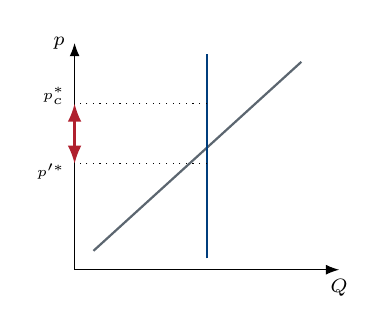
\begin{tikzpicture}[scale=0.48]
        \draw[-{Latex}] (0,0) -- (7,0) node[below, font=\scriptsize]{$Q$};
        \draw[-{Latex}] (0,0) -- (0,6) node[left, font=\scriptsize]{$p$};
        \draw[wugray, thick] (0.5,0.5) -- (6,5.5);
        \draw[wublue, thick] (3.5,0.3) -- (3.5,5.7);
        \draw[dotted] (3.5,4.4) -- (0,4.4);
        \draw[dotted] (3.5,2.8) -- (0,2.8);
        \draw[wured, thick, {Latex}-{Latex}] (0,2.8) -- (0,4.4);
        \node[left, font=\tiny] at (0,4.6) {$p_c^*$};
        \node[left, font=\tiny] at (0,2.6) {$p'^*$};
      \end{tikzpicture}\\[0.3em]
      Quantity can't change --- consumers bear \textbf{100\%} of the burden.
    \end{column}
    \begin{column}{0.5\textwidth}
      \centering \textbf{Perfectly elastic demand}\\[0.2em]
      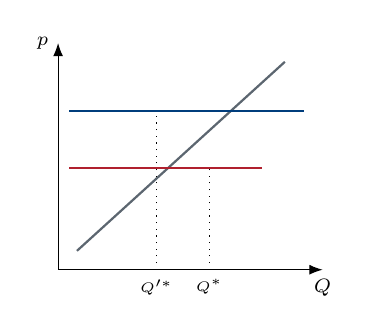
\begin{tikzpicture}[scale=0.48]
        \draw[-{Latex}] (0,0) -- (7,0) node[below, font=\scriptsize]{$Q$};
        \draw[-{Latex}] (0,0) -- (0,6) node[left, font=\scriptsize]{$p$};
        \draw[wugray, thick] (0.5,0.5) -- (6,5.5);
        \draw[wublue, thick] (0.3,4.2) -- (6.5,4.2);
        \draw[wured, thick] (0.3,2.7) -- (5.4,2.7);
        \draw[dotted] (2.6,0) -- (2.6,4.2);
        \draw[dotted] (4,0) -- (4,2.7);
        \node[below, font=\tiny] at (2.6,0) {$Q'^*$};
        \node[below, font=\tiny] at (4,0) {$Q^*$};
      \end{tikzpicture}\\[0.3em]
      Consumer price can't change --- producers bear \textbf{100\%} of the burden.
    \end{column}
  \end{columns}
  \vspace{0.4em}
  
  \alert{The side of the market with the \emph{less elastic} response bears more of the tax --- regardless of who writes the check.}
\end{frame}

\begin{frame}{Elasticity Determines Incidence}
  \begin{itemize}
    \item In theory, incidence does \emph{not} depend on who is statutorily required to pay --- a tax on sellers and an equivalent tax on buyers have the same economic incidence.
    \item What matters is the \textbf{relative elasticity of supply and demand}:
  \end{itemize}
  \[
    \varepsilon_D = \frac{p_c}{D}\frac{dD}{dp_c}, \qquad \varepsilon_S = \frac{p}{S}\frac{dS}{dp}
  \]
  \vspace{0.3em}
  \begin{alertblock}{Application: excise taxes in Austria}
    Austria taxes tobacco, alcohol, mineral oil, and (since 2022) CO\textsubscript{2} emissions via excise duties. Demand for cigarettes and heating fuel is famously \textbf{inelastic} in the short run --- so standard incidence theory predicts these taxes fall mostly on \emph{consumers}, not producers.
  \end{alertblock}
\end{frame}

\begin{frame}{The Equity--Efficiency Trade-off, Revisited}
  \small
  A progressive income tax has two effects:
  \begin{enumerate}
    \item \textbf{Equity gain}: reduces income inequality.
    \item \textbf{Efficiency loss}: people may work less when income is taxed --- if they care about \emph{net}, not gross, pay.
  \end{enumerate}
  \vspace{0.3em}
  The size of the efficiency loss is governed by the \textbf{elasticity of labor supply} (Lecture 2). Governments can dampen it by using tax revenue to subsidize goods complementary to working, such as child care.
  \vspace{0.3em}

  \(\Rightarrow\) ``How Can Scandinavians Tax So Much?'' (Kleven, 2014) --- high-tax Nordic countries also invest heavily in making work easy (child care, low-distortion consumption taxes), which is part of how they sustain such high tax revenue with limited efficiency loss.\\
  \srcnote{Kleven, H., \emph{Journal of Economic Perspectives} 28(4), 2014, cited in Leenders, Part IV.}
\end{frame}

% =============================================================
\section{4.3 Measuring the Fairness of Tax Systems}

\begin{frame}{Average vs.\ Marginal Tax Rates}
  \begin{block}{Marginal tax rate}
    The share of the \emph{next euro} of taxable income paid in tax.
  \end{block}
  \begin{block}{Average tax rate}
    Total tax paid, divided by total (gross) income --- a weighted average of all the marginal rates paid along the way.
  \end{block}
\end{frame}

\begin{frame}{Austria's 2026 Income Tax Brackets}
 \begin{table}
 	\centering
 	\begin{tabular}{@{}lr@{}}
 		\toprule
 		\textbf{ } & \textbf{Tax rate} \\
 		\midrule
 		13.539 und darunter & 0\,\% \\
 		über 13.539 bis 21.992 & 20\,\% \\
 		über 21.992 bis 36.458 & 30\,\% \\
 		über 36.458 bis 70.365 & 40\,\% \\
 		über 70.365 bis 104.859 & 48\,\% \\
 		über 104.859 bis 1.000.000 & 50\,\% \\
 		über 1.000.000\textsuperscript{1)} & 55\,\% \\
 		\bottomrule
 	\end{tabular}
 
 \end{table}
  
  
  \vspace{0.5em}
   \small
  The 55\% top bracket is a temporary surcharge. Brackets are progressive: each additional euro is taxed at a higher rate than the last.\\
 
\end{frame}

 

\begin{frame}{Worked Example: Lena's Tax Bill}
	\footnotesize
	Lena has taxable income of \texteuro{}80,000. Walking up the bracket schedule:
	\[
	(\text{\texteuro}8{,}453 \times 0.20) + (\text{\texteuro}14{,}466 \times 0.30) + (\text{\texteuro}33{,}907 \times 0.40) + (\text{\texteuro}9{,}635 \times 0.48) = \text{\texteuro}24{,}218.00
	\]
	Her disposable income: 80,000-24,218=55,782
	\vspace{0.3em}
	\begin{itemize}
		\item Lena's \textbf{marginal} tax rate is \textbf{48\%} --- the rate on her next euro earned.
		\item Lena's \textbf{average} tax rate is \(\text{\texteuro}24{,}218.00 / \text{\texteuro}80{,}000 = \mathbf{30.3\%}\).
	\end{itemize}
	\vspace{0.3em}

	The gap between the two --- 48\% vs.\ 30.3\% --- is entirely due to progressivity: the first \texteuro{}13,539 was tax-free, and every bracket below her marginal one was taxed at a lower rate.
\end{frame}

\begin{frame}{Vertical and Horizontal Equity}
  \begin{block}{Vertical equity}
    Groups with more resources should pay higher taxes than groups with fewer resources.
  \end{block}
  \begin{block}{Horizontal equity}
    Individuals who are similar, but make different choices, should be treated the same by the tax system.
  \end{block}
  \vspace{0.3em}
  \begin{itemize}
    \item A \textbf{progressive} system: average tax rates \emph{rise} with income.
    \item A \textbf{proportional} (flat) system: average tax rates are \emph{constant}.
    \item A \textbf{regressive} system: average tax rates \emph{fall} with income.
  \end{itemize}
\end{frame}

\begin{frame}{When ``Fair'' Causes a Riot}
  \small
  In March 1990, rioters in London set fire to parked cars and smashed storefronts, injuring more than 400 people. The cause: Margaret Thatcher's proposal to replace property taxes with a \textbf{poll tax} --- a flat charge levied \emph{equally} on every adult, rich or poor.
  \vspace{0.3em}
  \begin{alertblock}{Why it provoked outrage}
    The tax burden shifted away from wealthy property owners and onto poorer citizens who hadn't previously paid property tax at all --- a textbook violation of \textbf{vertical equity}. Thatcher was ousted as Conservative leader soon after; the tax was abandoned.
  \end{alertblock}
  \vspace{0.3em}
 
  (England's last attempt at such a tax, in 1381, ended with the beheading of several prominent officials.)\\

\end{frame}

\begin{frame}{Austria's Own Fairness Debate: \emph{Kalte Progression}}
  \footnotesize
  \begin{block}{The problem}
    With fixed, progressive brackets, \textbf{inflation} pushes people into higher brackets even when their \emph{real} income hasn't grown --- a stealth tax increase known as \emph{kalte Progression} (bracket creep).
  \end{block}
  \vspace{0.3em}
  \begin{itemize}
    \item Effective 1 January 2023, Austria began \textbf{automatically indexing} tax brackets to inflation: two-thirds of the inflation adjustment happens automatically by law each year; the remaining third is allocated at the government's discretion via a separate ``\emph{Progressionsabgeltungsgesetz}.''
    \item The top \texteuro{}1{,}000{,}000 / 55\% bracket is \emph{excluded} from indexation.
  \end{itemize}
 
 
 \end{frame}

% =============================================================
\section{4.4 Defining the Income Tax Base}

\begin{frame}{The Haig-Simons Comprehensive Income Definition}
  \begin{block}{Haig-Simons income}
    Taxable resources = an individual's \emph{ability to pay} = total consumption during the year \(+\) any increase in wealth.
  \end{block}
  \vspace{0.3em}
  \begin{itemize}
    \item In principle, comprehensive income improves \emph{both} vertical equity (all resources are taxed, however received) \emph{and} horizontal equity (the form compensation takes shouldn't matter).
    \item In practice, every real tax system deviates from this ideal --- the question is whether each deviation is justified.
  \end{itemize}
  \srcnote{Gruber, \emph{Public Finance and Public Policy}, \S18.4.}
\end{frame}

\begin{frame}{Austria vs.\ the US: In-Kind Compensation}
  \begin{itemize}
    \item The classic Haig-Simons violation in th US: employer-provided \textbf{health insurance} is not taxed as income, even though it clearly raises a worker's ability to consume.
    \item Austria takes a stricter approach for many in-kind benefits: the \emph{Sachbezugswerteverordnung} taxes the value of a company car, subsidized housing, and other in-kind perks as part of wage income.
  \end{itemize}

 
\end{frame}

\begin{frame}{Deviations for Ability-to-Pay and Earning Costs}
  \small
  \begin{itemize}
    \item \textbf{Ability-to-pay deviations}: Austria's \emph{außergewöhnliche Belastungen} (extraordinary burden deductions) let taxpayers deduct large, involuntary costs --- medical expenses, disaster losses --- on the same logic as Gruber's ``fire damage'' example: these expenditures aren't really \emph{consumption}, so they shouldn't count as ability to pay.
    \item \textbf{Cost-of-earning-income deviations}: Austria's \emph{Werbungskosten} let workers deduct job-related expenses, including the \emph{Pendlerpauschale} (commuter allowance, Lecture 1) --- the same logic as deducting business costs from Haig-Simons income.
  \end{itemize}
  \vspace{0.3em}
  \centering
  Both are easy to justify in principle --- and hard to draw a clean line around in practice (was that lunch a business cost, or consumption?).
\end{frame}

\begin{frame}{Housing}
  \footnotesize
  \begin{itemize}
    \item Whether you rent or own, you consume \texteuro{}X/month of housing services --- your \emph{imputed rental value}. A true Haig-Simons tax would treat renters and owners identically.
    \item The \textbf{US} does not tax imputed rental income, \emph{but} lets owners deduct mortgage interest --- a large, one-sided subsidy to owning (\(\approx\)\texteuro{}80bn/year in forgone US federal revenue)
    \item Empirical research finds little evidence that home ownership has positive social benefits

    Austria   taxes owners and renters rather symmetrically  
 
  \end{itemize}
\end{frame}

\begin{frame}{Deductions vs.\ Credits}
  \begin{block}{Tax deduction}
    Reduces \emph{taxable income} --- its value to the taxpayer is \(\$(1-t)\) per euro, so it's worth \emph{more} to people in higher brackets.
  \end{block}
  \begin{block}{Tax credit}
    Reduces \emph{tax owed} directly --- worth the same to everyone, regardless of bracket, and thus more progressive.
  \end{block}
  \vspace{0.3em}
   
  A \textbf{refundable} credit goes further still: it pays out even to people who owe little or no tax --- turning the tax system into a delivery mechanism for cash transfers to low earners.
\end{frame}

\begin{frame}{Austria's Own Refundability Debate: \emph{Familienbonus Plus}}
  \footnotesize
  Introduced in 2019 as a tax \textbf{credit} (not a deduction) for families with children.
  \begin{itemize}
    \item 2024 value: \texteuro{}2{,}000.16/year per child under 18; \texteuro{}700.08/year per child 18 or older.
    \item Because it's a credit against tax owed, it delivers \emph{nothing} to a parent who owes little or no income tax --- exactly the refundability problem the US Child Tax Credit debate raises.
    \item Austria's partial fix: the \emph{Kindermehrbetrag} (2024: \texteuro{}700/child) tops up low earners who claim the sole-earner/single-parent credit, closing the gap between their (near-zero) tax liability and \texteuro{}700.
  \end{itemize}
  \vspace{0.3em}
  \centering
  \alert{Discussion:} does the Kindermehrbetrag fully solve the vertical-equity problem of a non-refundable credit, or only partly?\\
  \srcnote{Bundeskanzleramt; BMF, Familienbonus Plus \& Kindermehrbetrag (2024).}
\end{frame}

\begin{frame}{Tax Expenditures}
  \begin{block}{Tax expenditures}
    Revenue the government forgoes through special exclusions, deductions, credits, or preferential rates --- functionally equivalent to direct spending, just routed through the tax code instead of the budget.
  \end{block}
  \vspace{0.3em}
  \centering
  In the US, tax expenditures total over \texteuro{}1 trillion/year --- more than 40\% of total tax revenue. Every deduction and credit on the last several slides (Familienbonus Plus, Werbungskosten, außergewöhnliche Belastungen) is, by this definition, an Austrian tax expenditure too.\\
  \srcnote{Gruber, \emph{Public Finance and Public Policy}, \S18.5, citing U.S.\ Department of the Treasury (2021a).}
\end{frame}

% =============================================================
\section{The Rise of the Fiscal State}

\begin{frame}{How Did We Get Progressive Taxation?}
  \small
  \begin{itemize}
    \item Top marginal income-tax rates were in the single digits almost everywhere before 1900 --- then rose sharply, above all in the US, UK, Sweden, Germany, and France, from the 1910s onward.
    \item \textbf{World War I} acted as the catalyst: many countries raised top rates on income and inheritances explicitly as a ``conscription of capital'' to match the conscription of soldiers.
    \item The wartime rate hikes only \emph{stuck} because of lasting technological and institutional changes: employer-based withholding, and --- eventually --- the end of bank secrecy.
  \end{itemize}
  \vspace{0.3em}
  \begin{alertblock}{Austria's own version of that last point}
    Austria was long known for strict \emph{Bankgeheimnis} (bank secrecy). That changed with the OECD's Common Reporting Standard: Austria began automatically exchanging account data with foreign tax authorities starting September 2017.
  \end{alertblock}
  \srcnote{Leenders, Part IV, citing Piketty, \emph{Capital and Ideology} (2020); Gemeinsamer Meldestandard-Gesetz (GMSG), effective 2016--2017.}
\end{frame}

\begin{frame}{The Long-Run Fall in Top Income Shares: L-Shaped}
  \begin{center}
    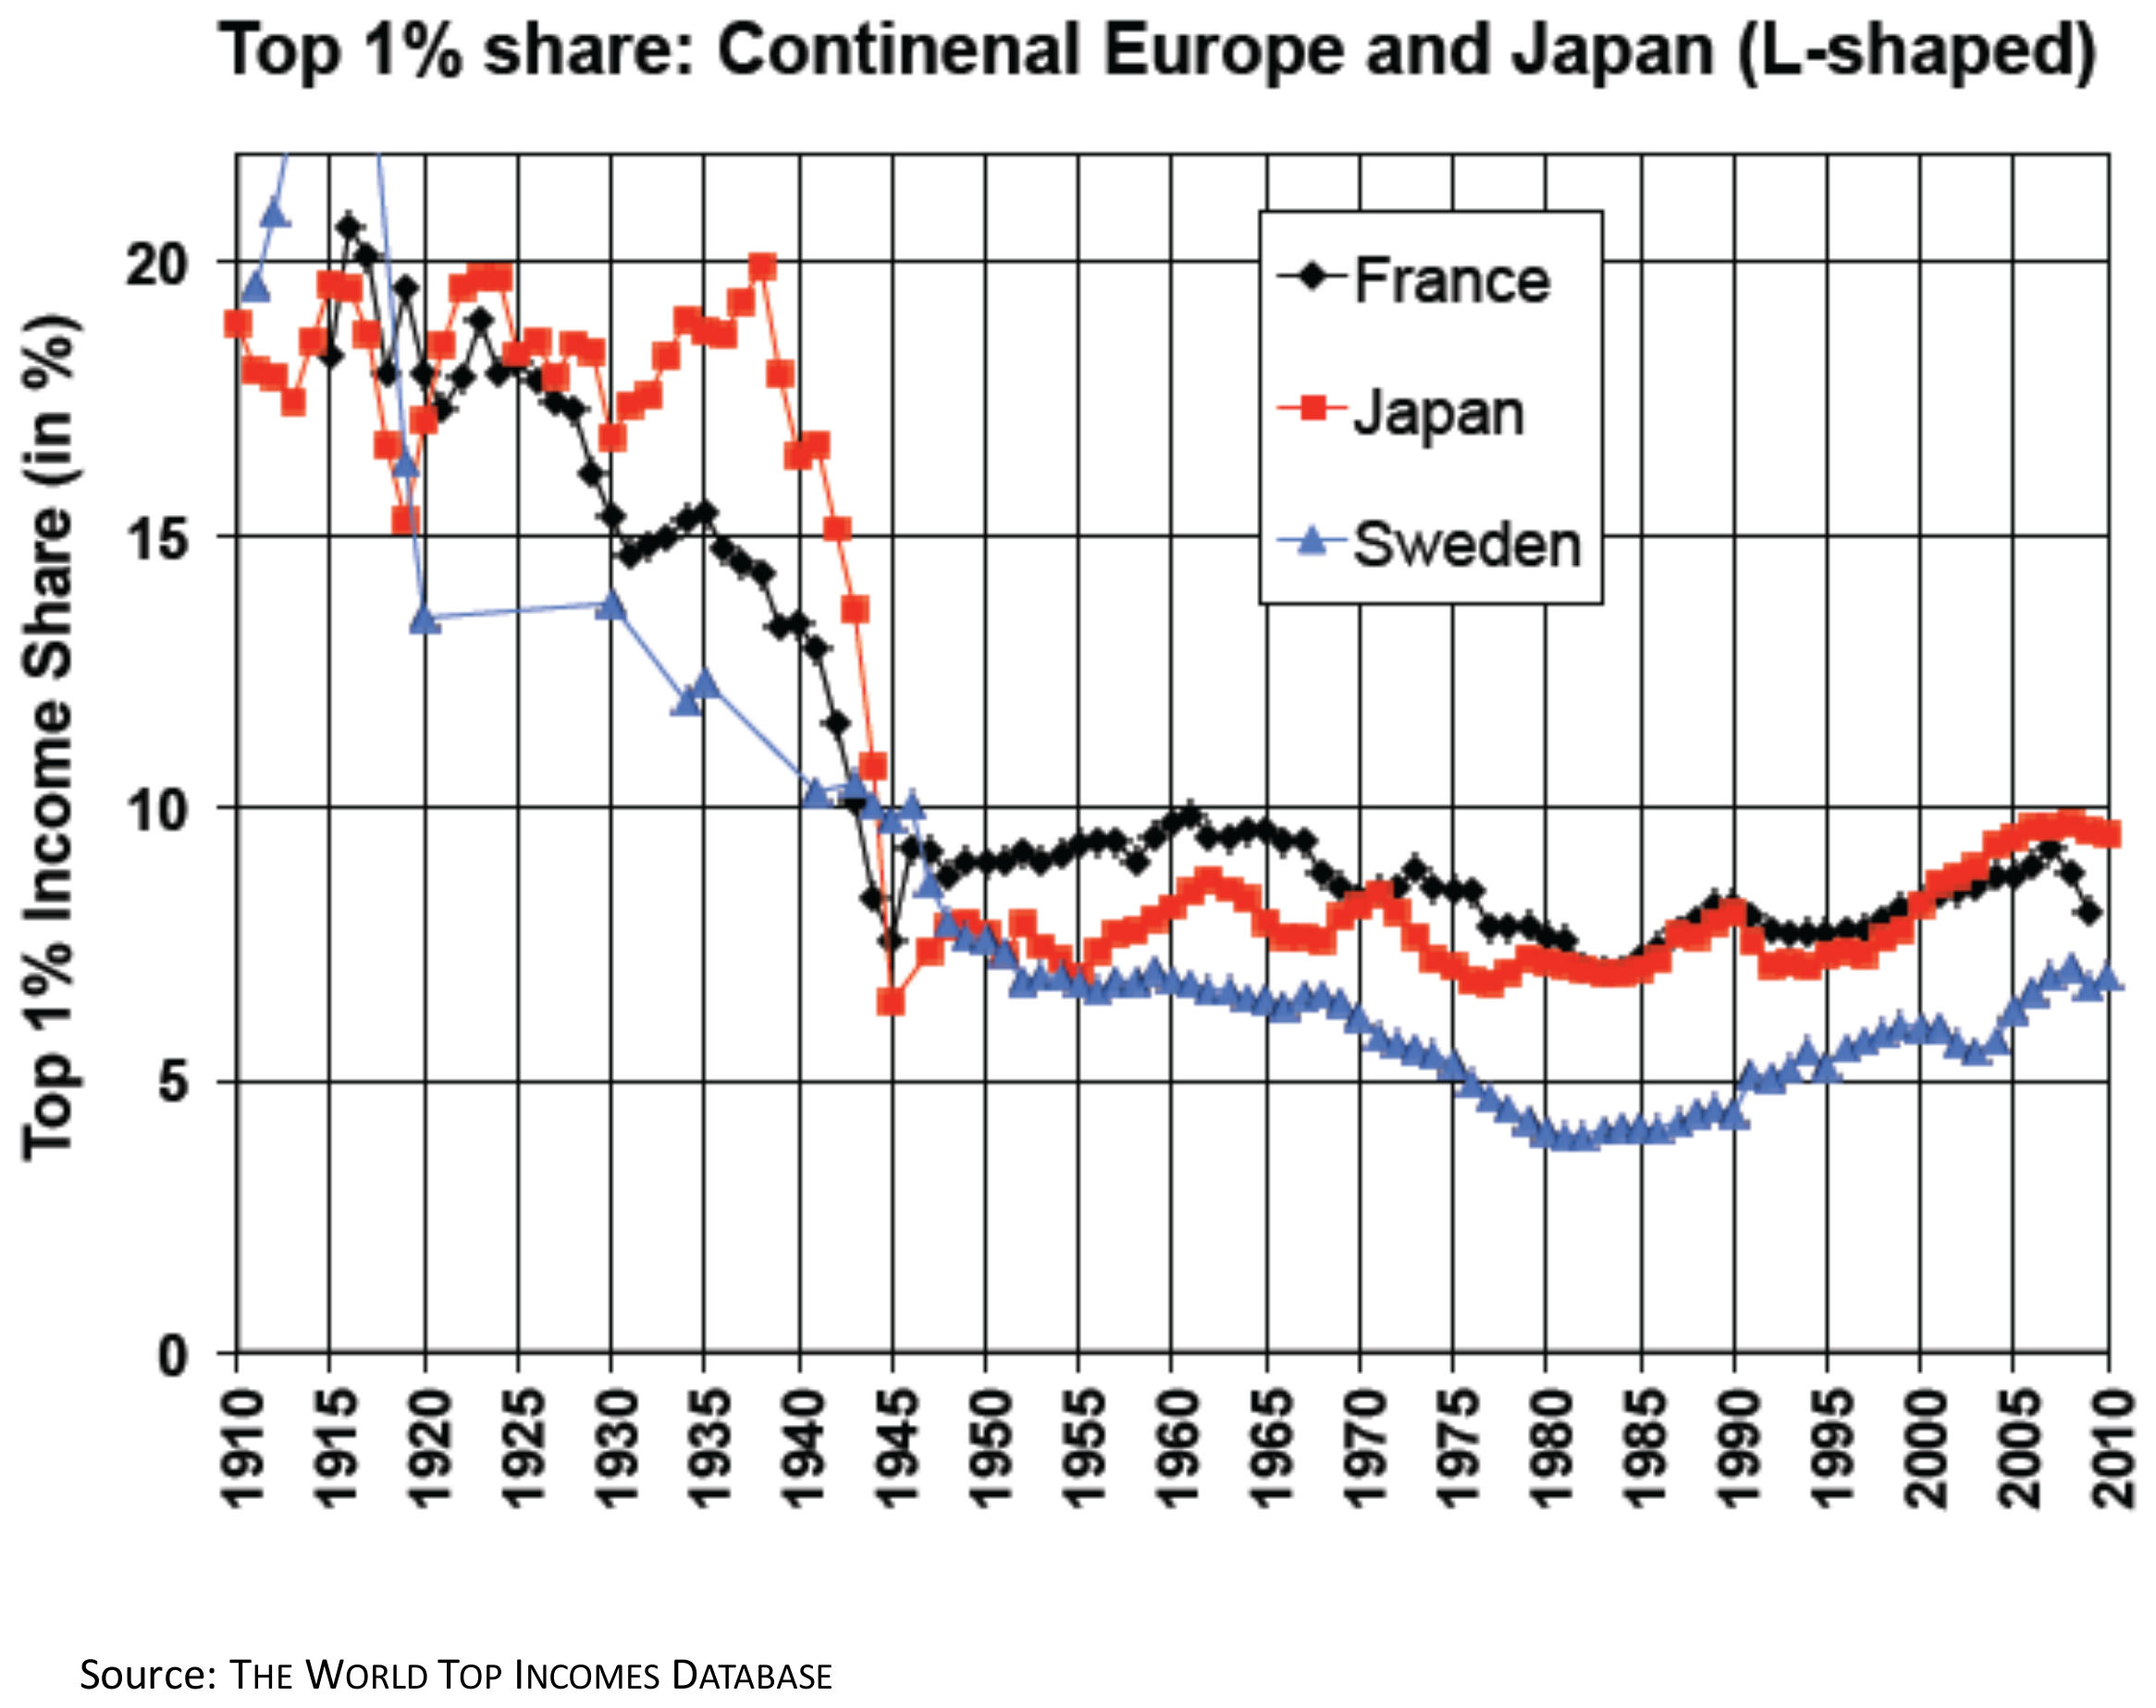
\includegraphics[height=4.9cm]{figures/top1pct_europe_japan_lshaped.png}
  \end{center}
  \centering
  \footnotesize
  The rate hikes on the previous slide show up directly in the data: top 1\% income shares in France, Japan, and Sweden collapsed from \(\approx\)18--20\% before WWII to \(\approx\)4--8\% by the 1970s--80s --- and \textbf{stayed low} since.\\
  \srcnote{World Top Incomes Database / WID.world.}
\end{frame}

\begin{frame}{...vs.\ U-Shaped: English-Speaking Countries}
  \begin{center}
    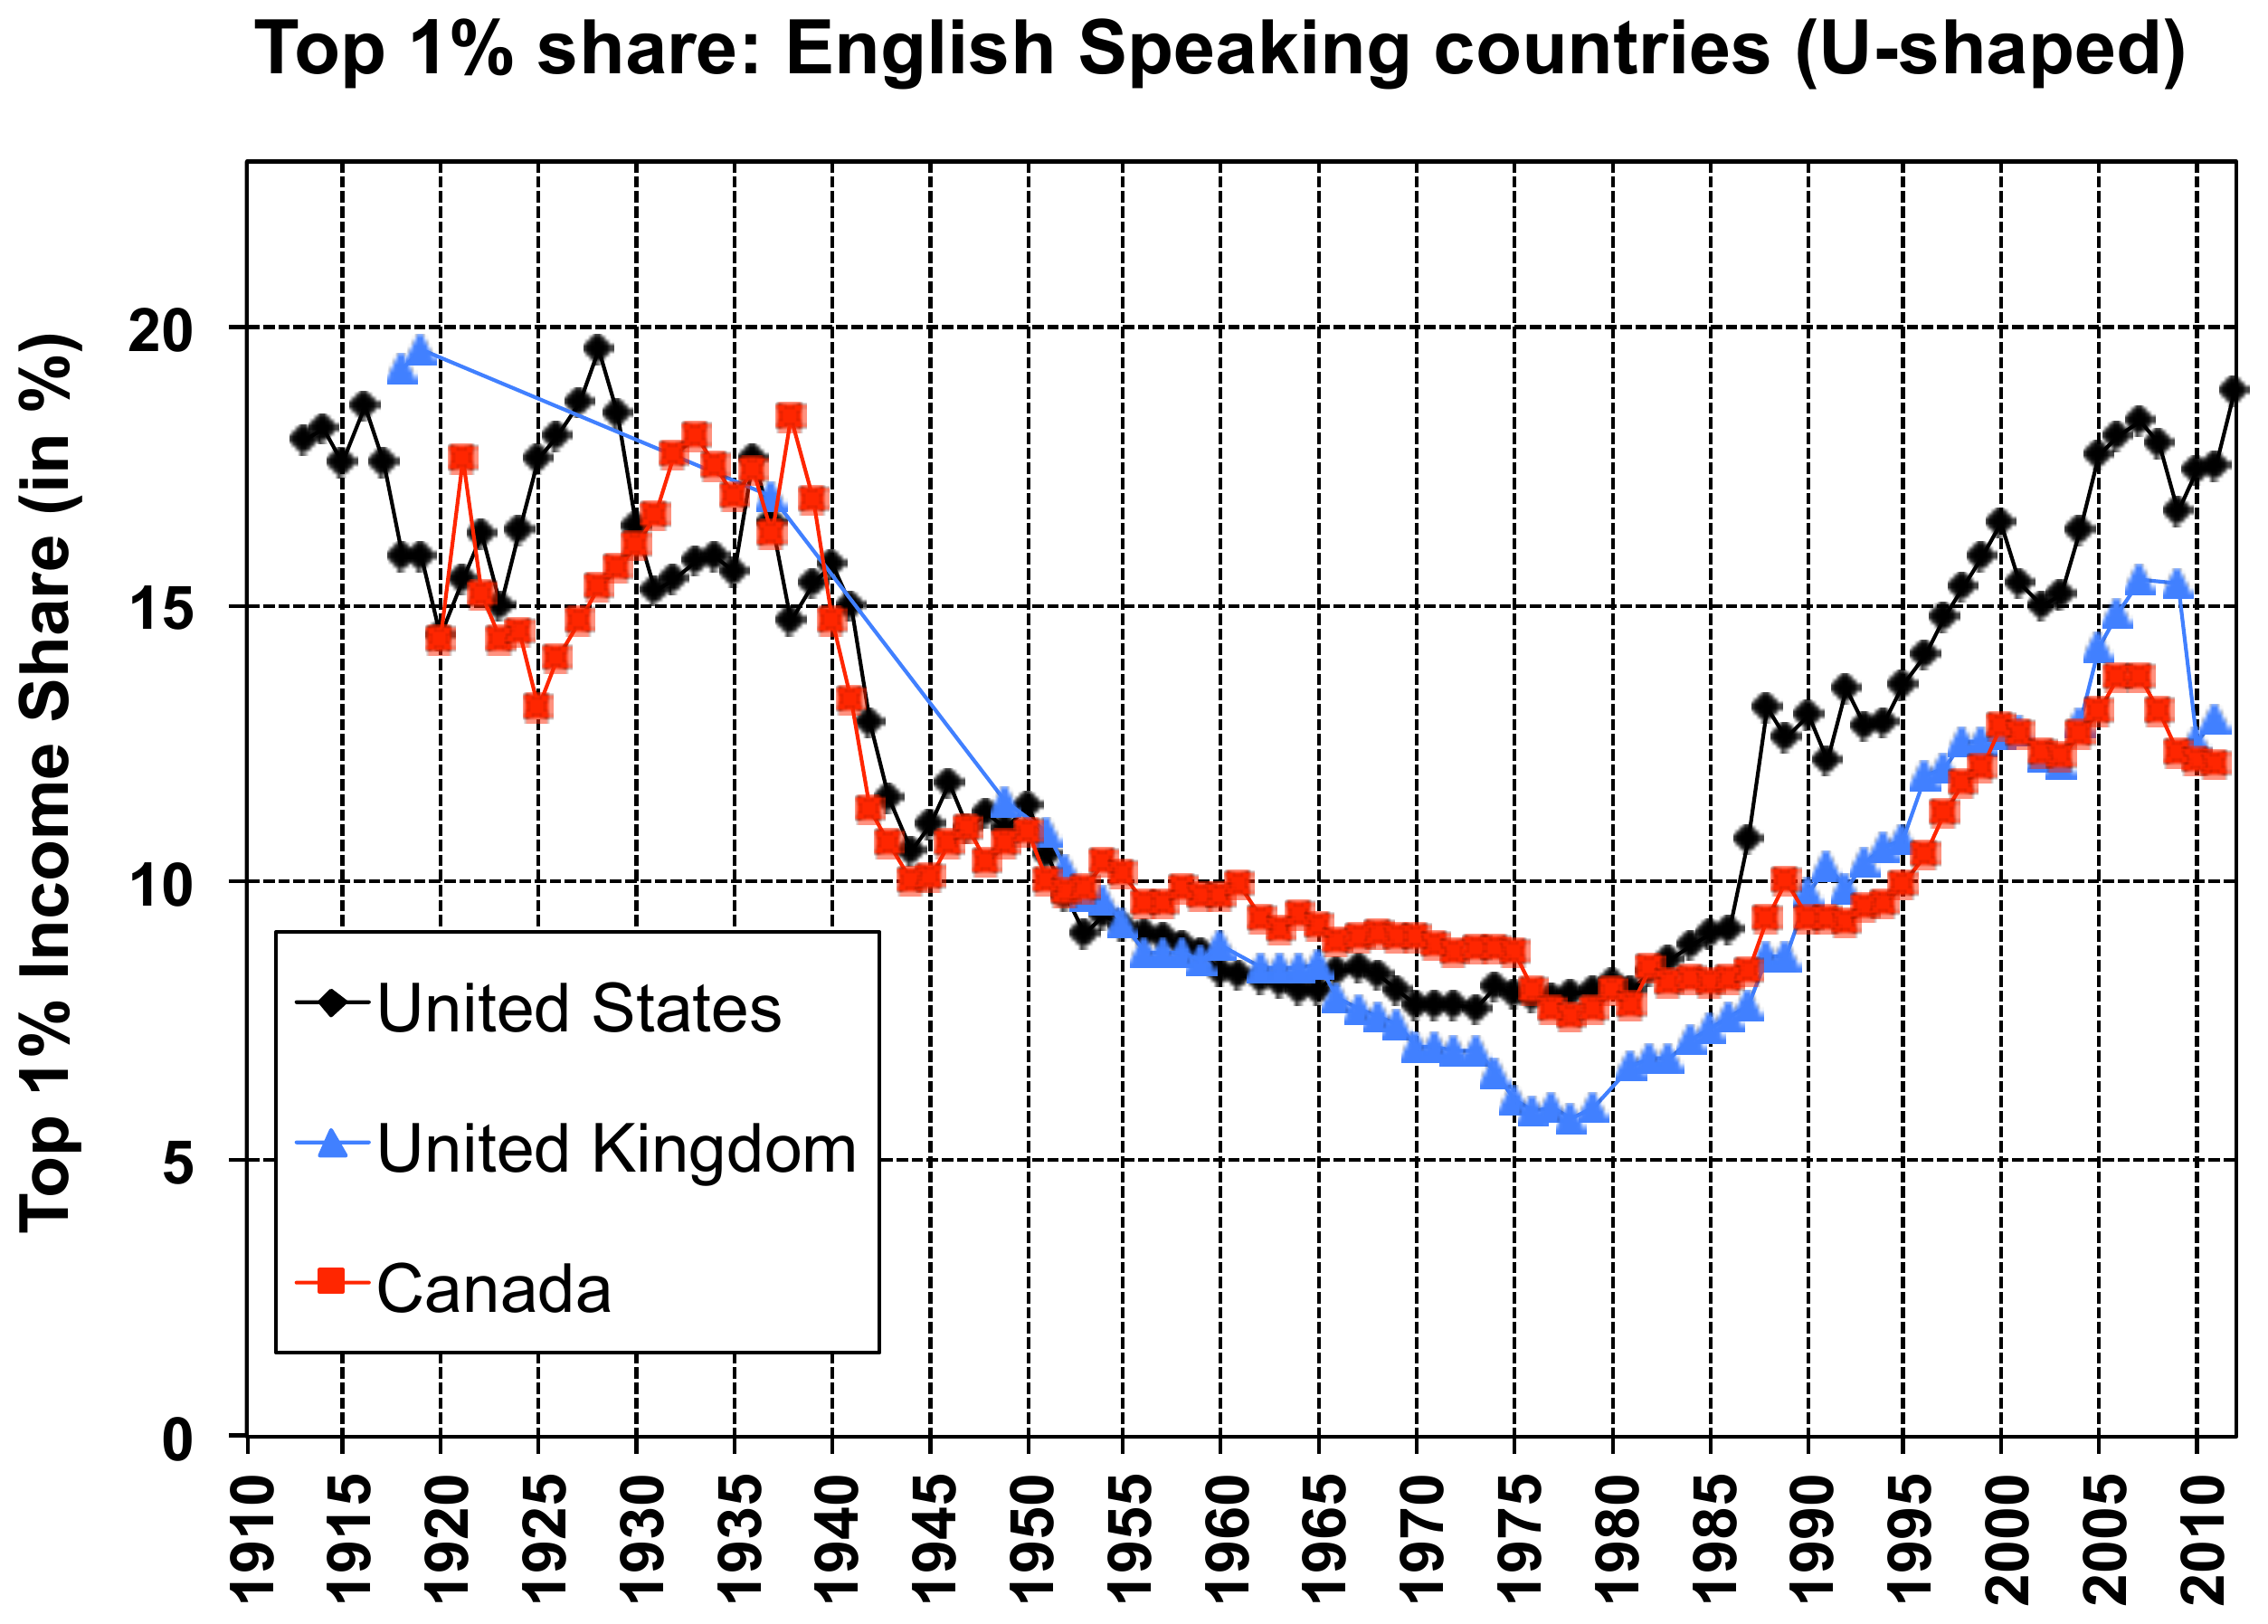
\includegraphics[height=2.85cm]{figures/top1pct_english_speaking_ushaped.png}
  \end{center}
  \footnotesize
  The US, UK, and Canada saw an equally sharp WWII-era collapse --- but then \textbf{rebounded} close to pre-war levels by the 2010s.
  \vspace{0.3em}
  \begin{alertblock}{Why the difference?}
    Piketty, Saez \& Stantcheva (2014) link this directly to \emph{tax} policy: countries that cut top marginal rates the most after 1980 (the US, UK) saw the largest rebound in top income shares; countries that kept rates comparatively high (France, Germany, much of Continental Europe) saw much smaller rebounds.
  \end{alertblock}
  \srcnote{World Top Incomes Database / WID.world; Piketty, Saez \& Stantcheva, ``Optimal Taxation of Top Labor Incomes,'' \emph{AEJ: Economic Policy} 6(1), 2014.}
\end{frame}

\begin{frame}{Why This History Matters}
  \begin{itemize}
    \item The rise in top rates on the wealthy over the twentieth century is a major part of the story behind the dramatic \emph{fall} in income and wealth inequality across the same period (Lecture 1).
    \item Total tax revenue as a share of national income rose alongside it, from roughly 5--10\% (1870) to 30--55\% (today) across today's rich democracies --- with the US consistently at the \emph{low} end of that range and the Nordic countries at the \emph{high} end.
  \end{itemize}
  \vspace{0.3em}
  \centering
  \alert{This isn't ancient history --- it's the direct backdrop to the debates in this lecture: what should be taxed, how progressively, and how the tax base should be defined.}\\
  \srcnote{Leenders, Part IV, citing Piketty (2020) and long-run OECD/WID revenue series.}
\end{frame}

\section{4.5 The Appropriate Unit of Taxation}

\begin{frame}{Whose Income Do We Tax? Pick Two of Three}
	\small
	Suppose a tax system had to satisfy three goals at once:
	\begin{itemize}
		\item \textbf{Progressivity}: marginal tax rates rise as income rises.
		\item \textbf{Across-family horizontal equity}: families with equal total income pay equal tax.
		\item \textbf{Across-marriage horizontal equity}: tax burdens are \emph{marriage neutral} --- unaffected by whether two people wed.
	\end{itemize}
	\vspace{0.3em}

		All three seem reasonable. It is \textbf{impossible} to satisfy all three simultaneously --- any progressive tax system taxing couples on some notion of joint income must give up at least one.


\end{frame}

\begin{frame}{Worked Example: Two Couples, Same Income}
	\footnotesize
	A stylized progressive schedule: 10\% up to \texteuro{}20{,}000; 20\% up to \texteuro{}80{,}000; 30\% above \texteuro{}80{,}000 (illustrative only --- not Austria's actual schedule).
	\vspace{0.3em}
	\begin{center}
		\begin{tabular}{@{}lccc@{}}
			\toprule
			& \textbf{Individual incomes} & \textbf{Tax, filed individually} & \textbf{Tax, filed as a family} \\
			\midrule
			Yasmin \& Doug & \texteuro{}140{,}000 + \texteuro{}10{,}000 & \texteuro{}33{,}000 & \texteuro{}35{,}000 \\
			Jan \& Elena & \texteuro{}75{,}000 + \texteuro{}75{,}000 & \texteuro{}26{,}000 & \texteuro{}35{,}000 \\
			\bottomrule
		\end{tabular}
	\end{center}
	\vspace{0.3em}
	Both couples earn \texteuro{}150{,}000 combined.
	\begin{itemize}
		\item \textbf{Individual filing}: Yasmin \& Doug pay \texteuro{}7{,}000 \emph{more} than Jan \& Elena, despite equal family income --- violates across-family equity.
		\item \textbf{Family filing}: both couples pay \texteuro{}35{,}000 --- equal treatment, but \emph{both} now pay more than they did unmarried --- a \textbf{marriage tax}.
	\end{itemize}

\end{frame}

\begin{frame}{Why the Trade-off Is Unavoidable}
	\small
	\begin{itemize}
		\item Under \textbf{individual} filing, rising marginal rates mean two-earner couples with similarly-sized incomes (Jan \& Elena) pay less than one-earner-dominant couples (Yasmin \& Doug) with the same total --- that's the equity violation.
		\item Under \textbf{family} filing, combining incomes pushes the secondary earner's earnings on top of the primary earner's --- Doug's first \texteuro{}10{,}000, taxed at 10\% individually, gets taxed at 30\% once merged with Yasmin's income. That's the marriage tax.
		\item The \emph{only} escape from both problems at once is a flat (proportional) tax --- which gives up progressivity, the first goal.
	\end{itemize}
	\vspace{0.3em}
	\centering

\end{frame}



\begin{frame}{Marriage Tax in Austria}

	\begin{itemize}
		\item Austria taxes spouses \textbf{individually}, not as a family unit --- and has done so since 1973, when a family-law reform replaced the previous household-taxation system.
		\item Because each partner's tax bracket depends only on \emph{their own} income, getting married changes \textbf{nobody's} tax bill by itself --- Austria's system is marriage-neutral 
	
 
		\item The \emph{Alleinverdienerabsetzbetrag} (sole-earner credit) gives a small, means-tested credit to one-earner couples/families with children when the lower-earning partner's income stays below a threshold 
 
\end{itemize}
\end{frame}

\begin{frame}{The Unit of Taxation Around the World}
	\footnotesize
	\begin{center}
		\begin{tabular}{@{}lp{7.5cm}@{}}
			\toprule
			\textbf{System} & \textbf{OECD countries} \\
			\midrule
			Individual taxation & 19 countries, \textbf{including Austria} \\
			Family taxation with income splitting & France, Germany, Luxembourg, Portugal, Switzerland (mostly generates marriage \emph{subsidies}) \\
			``Pure'' family taxation (no splitting) & United States, Ireland, Norway \\
			\bottomrule
		\end{tabular}
	\end{center}
	\vspace{0.3em}
	\centering

\end{frame}
% =============================================================
\section{The Distribution of the Tax Burden}

\begin{frame}{Who Actually Pays the Taxes?}
  \begin{itemize}
    \item Rather than asking how a \emph{hypothetical} tax change would affect prices (incidence theory), a newer research tradition (Saez \& Zucman, 2019, and successors) asks: given the tax system \emph{as it exists}, what share of everyone's income actually goes to tax, by income rank?
    \item Applied to the Netherlands, Italy, France, and the US, this research finds effective tax rates that \textbf{rise} through the middle of the distribution --- then \textbf{flatten or fall} at the very top.
  \end{itemize}
  \vspace{0.3em}
 
  The progressivity we build into income-tax \emph{brackets} doesn't automatically show up in the effective rate actually paid, once every tax is counted. 
  \ 
\end{frame}

\begin{frame}{Four Insights on Who Pays}
 
  \begin{enumerate}
    \setlength{\itemsep}{1pt}
    \item \textbf{Income taxes} are progressive for the bottom 90\% of earners, but play only a minor role at the very top --- where income increasingly comes from capital, not wages.
    \item \textbf{Corporate taxes} act as a kind of minimum tax on the rich, since a large share of top-end income flows through corporate ownership.
    \item \textbf{Consumption taxes} hit lower-income households hardest, because they consume a larger \emph{share} of their income than the wealthy do.
    \item \textbf{Payroll taxes} are levied only on labor income --- and labor income's share of total income \emph{falls} as you move up the distribution, which is regressive.
  \end{enumerate}

\end{frame}

\begin{frame}[fragile]{Try It Yourself: Design Your Own Tax System}
  \small
  Saez \& Zucman built an interactive tool around the same distributional data from the last two slides --- it lets you set tax rates by income group and see the revenue and distributional consequences in real time.
  \vspace{0.5em}
  \begin{center}
    \Large \url{https://taxjusticenow.org/#makeYourOwnTaxPlan}
  \end{center}
  \vspace{0.5em}
  \centering
  \alert{In-class exercise:} pick a distributional goal (e.g.\ ``flat effective rate for everyone'' or ``restore 1950s-style progressivity at the top'') and see what tax rates it actually takes to get there.\\
  \srcnote{Saez \& Zucman, \emph{taxjusticenow.org}, companion site to \emph{The Triumph of Injustice} (2019).}
\end{frame}

% =============================================================




\begin{frame}[standout]
  Thank you!\\
  \vspace{0.5em}
  \small Questions and discussion
\end{frame}

\end{document}
